\part{Ricerca e ordinamento}

\chapter{Problema della ricerca}
Nell'informatica esistono alcuni problemi particolarmente rilevanti. Uno tra questi è il problema della ricerca di un elemento in un insieme di
dati.

Definiamo più formalmente tale problema descrivendone l’input e l’output:
\begin{itemize}
    \item \textbf{Input}: una lista di numeri \verb|n| numeri interi ed un valore \verb|v| da ricercare.
    \item \textbf{Output}: un indice \verb|i| tale che \verb|lista[i]=v| oppure un particolare valore \verb|Nome| se \verb|v| non è presente nella lista.
\end{itemize}

\section{Ricerca sequenziale}

Un primo semplice algoritmo è basato sulla seguente idea. Ispezioniamo uno alla volta gli elementi del vettore, confrontando ciascun elemento con \verb|v|. Se troviamo \verb|v| restituiamo il suo indice, terminando l’algoritmo. Se \verb|v| non è contenuto nel vettore, alla fine della scansione
restituiamo None.

Da qui ne ricaviamo il seguente codice:
\begin{lstlisting}[language=Python]
        def ricercaSeq(A,v):
            n=len(A)
            for i in range(n):
                if A[i]==v:
                    return i
            return None
    \end{lstlisting}
    
Questo algoritmo ha un costo di:
\begin{itemize}
    \item $\Theta(n)$ nel caso peggiore (quando v non è presente nella lista);
    \item $\Theta(1)$ nel caso migliore (quando v è il primo elemento).
\end{itemize}

In queste situazioni diremo che il costo dell'algoritmo in generale è un $O(n)$, per evidenziare il concetto che l'algoritmo non può risultare peggiore di quella complessità.

Nei casi, come questo, in cui non sia possibile determinare un valore stretto per il costo computazionale, ed in cui il caso migliore e quello  peggiore si discostano, è naturale domandarsi quale sia il costo computazionale dell'algoritmo nel \textbf{caso medio}.

\subsubsection{Caso medio dell'algoritmo}

Facciamo l’ipotesi che gli elementi del vettore siano distinti e che \verb|v| possa apparire con uguale probabilità in qualunque posizione, ossia che:
\begin{equation*}
    P\text{ (probabilità di trovare v nell'i-esima posizione )} = \frac{1}{n}
\end{equation*}

Allora il numero medio di iterazioni del ciclo è dato da:
\begin{equation*}
    \sum^n_{i=1}i\frac{1}{n}=\frac{1}{n}\frac{n(n+1)}{2}=\frac{n+1}{2}
\end{equation*}


Un’ipotesi alternativa è la seguente: supponiamo che tutte le possibili $n!$ permutazioni della sequenza di numeri siano equiprobabili.
Di queste, ve ne saranno un certo numero nelle quali \verb|v| appare in prima posizione, un certo numero nelle quali \verb|v| appare in seconda posizione, ecc.
Il numero medio di iterazioni del ciclo sarà di conseguenza: 

\begin{equation*}
    \sum^n_{i=1}i\frac{\text{numero di permutazioni in cui v è in posizione i}}{\text{numero totale di permutazioni}}
\end{equation*}

Ora, il numero di permutazioni nelle quali \verb|v| appare nella i-esima posizione è uguale al numero delle permutazioni di $n-1$ elementi, cioè $(n-1)!$ dato che fissiamo solo la posizione di uno degli n elementi.

\begin{equation*}
    \text{Numero medio di iterazioni}=\sum^n_{i=1}i\frac{(n-1)!}{n!}=\frac{1}{n}\sum^n_{i=1}i=\frac{n+1}{2}
\end{equation*}

Partendo da due diverse ipotesi di equiprobabilità abbiamo ottenuto lo stesso
risultato: il costo computazionale nel caso medio è $\Theta(n)$.


\section{Ricerca binaria}
Con la ricerca binaria è possibile progettare un algoritmo molto più efficiente nel caso in cui la sequenza degli elementi sia ordinata.

L'idea è la seguente. Si ispeziona l’elemento centrale della sequenza, se esso è uguale al valore cercato ci si ferma. Se il valore cercato è più piccolo si prosegue nella sola metà inferiore della sequenza, altrimenti nella sola metà superiore.

Ad ogni iterazione si dimezza il numero degli elementi su cui proseguire l’indagine. 
Infatti dopo $i$ iterazioni il numero di elementi su cui ricercare sarà $\frac{n}{2^i}$. Alla peggio ci si ferma quando per $i$ si ha $\frac{n}{2^i}=1$ vale a dire $2^i=n$ ovvero $i=\log n$.

Questo ci permette di capire perchè la ricerca binaria sia così efficiente: il numero di iterazioni cresce come $\log n$. 

\begin{lstlisting}[language=Python]
    def RB(A,v):
        a,b=0,len(A)-1
        while a<=b:
            m=(a+b)//2
            if A[m]==v:
                return m
            elif A[m]>v:
                b=m-1
            else:
                a=m+1
        return None
\end{lstlisting}

il costo computazionale è:
\begin{itemize}
    \item $\Theta(\log n)$ nel caso peggiore (quando l’elemento non è presente nel vettore);
    \item $\Theta(1)$ nel caso migliore (quando l'elemento si trova a metà del vettore).
\end{itemize}

Poiché caso migliore e caso peggiore non hanno lo stesso costo, valutiamo il costo computazionale del caso medio.

Domandiamoci ora quante siano le posizioni $n(i)$ raggiungibili alla i-esima iterazione: con una iterazione si raggiunge la sola posizione $\frac{n}{2}$, cioè $n(1)=2^0=1$; con due iterazioni si raggiungono le due posizioni $\frac{n}{4}$ e $3\frac{n}{4}$, cioè $n(2)=2^1=2$; con tre iterazioni si raggiungono le quattro posizioni $\frac{n}{8}$, $3\frac{n}{8}$, $5\frac{n}{8}$, $7\frac{n}{8}$, cioè $n(3)=2^2=4$.
    
In generale quindi, l’algoritmo di ricerca binaria esegue $i$ iterazioni se e solo se \verb|v| si trova in una delle $n(i)=2^{i-i}$ posizioni raggiungibili con tale numero di iterazioni.

Ricordando che la probabilità che l’elemento si trovi su una delle $n(i)$ posizioni toccate dalla i-esima iterazione è $\frac{n(i)}{n}$ (ossia $\frac{2^{i-1}}{n}$), il numero medio di iterazioni è:

\begin{equation*}
    \text{Numero medio di iterazioni}=\sum^{\log n}_{i=1}i\frac{n(i)}{n}=\frac{1}{n}\sum^{\log n}_{i=1}i2^{i-1}
\end{equation*}

e sapendo che $\sum^{\log n}_{i=1}i2^{i-1} = (k-1)2k + 1$ otteniamo:
\begin{equation*}
    \frac{i}{n} ((\log n - 1) * 2^{\log n} + 1) = \log n - 1 +\frac{1}{n}
\end{equation*}

Ossia, il numero medio di iterazioni si discosta per meno di un confronto dal numero massimo di iterazioni!

\chapter{Programmi ricorsivi}
In questo capitolo ci occuperemo di calcolare la complessità di programmi ricorsivi, ovvero programmi che richiamano se stessi, dove un problema viene suddiviso in sotto-problemi simili a quello originale, ma più semplici.

Iniziamo guardando qualche esempio, per poi imparare a calcolare il costo computazionale di un algoritmo ricorsivo.

\begin{example}
Calcoliamo in maniera ricorsiva il fattoriale di un numero n.
    \begin{lstlisting}[language=Python]
        def fatt(n):
            if n == 0: return 1
            return n*fatt(n-1)
    \end{lstlisting}
    
    Il costo computazionale di questo algoritmo dipende dai valori di n. Ovvero:
    $$T(n)=\begin{cases}
        \Theta(1)\hspace{0.5cm}\text{se}\hspace{0.5cm}n=0\\
        T(n-1)+\Theta(1)\hspace{0.5cm}\text{altrimenti}
    \end{cases}$$
    
    La complessità totale di questo algoritmo risulta essere dell'ordine $\Theta(n)$.
    
\end{example}

\begin{example}
    Ricerca di un elemento in un vettore ricorsivamente.
    \begin{lstlisting}[language=Python]
        def ricercaR(x, A):
            if A==[]: return False
            if A[0] == x: return True
            return ricercaR(x, A[1:])
    \end{lstlisting}
    
    Anche in questo caso il costo si divide in:
    $$T(n)=\begin{cases}
        \Theta(1)\hspace{0.5cm}\text{se}\hspace{0.5cm}n=0\\
        T(n-1)+\Theta(n)\hspace{0.5cm}\text{altrimenti}
    \end{cases}$$
    
    Il secondo $\Theta(n)$ dipende dal fatto che nella ricorsione viene richiamata una copia della lista origniale. Per tanto questa operazione di copia ha un costo che segue l'andamento di $\Theta(n)$. Si potrebbe risolvere questo problema considerando l'ultimo elemento della lista per poi eliminarlo quando viene passato come argomento della ricorsione. Il programma risultante sarebbe il seguente:
    \begin{lstlisting}[language=Python]
        def ricercaR(x, A):
            if A==[]: return False
            if A[-1] == x: return True
            A.pop()
            return ricercaR(x, A)
    \end{lstlisting}
    In questo modo il programma ha costo $\Theta(n)$, invece che $\Theta(n^2)$.
\end{example}

Ci tengo a ricordare che questi algoritmi sono solo introduttivi per prendere dimestichezza con il concetto di ricorsione. Infatti uno stesso programma iterativo risulterebbe molto più efficiente.

\begin{example}
    Quest'ultimo esempio riguarda il calcolo dell'i-esimo numero di Fibonacci.
    \begin{lstlisting}[language=Python]
        def fibR(n):
            if n<=1: return n
            reutrn fibR(n-1)+(n-2)
    \end{lstlisting}
    
    Questo è esattamente il tipo di programma ricorsivo che si vuole evitare. Scoprendo il costo computazionale dell'algoritmo capiremo il perchè:
    $$T(n)=\begin{cases}
        \Theta(1)\hspace{0.5cm}\text{se}\hspace{0.5cm}n\leq1\\
        T(n-1)+T(n-2)+\Theta(1)\hspace{0.5cm}\text{altrimenti}
    \end{cases}$$
    
    Che si risolve in una complessità dell'ordine $\Theta(2^n)$.
\end{example}

Ma come facciamo a calcolare la complessità di questi algoritmi?

\section{Equazioni di ricorrenza}
In questa sezione vengono forniti alcuni metodi per risolvere le equazioni di ricorrenza, indispensabili per il calcolo del tempo computazionale degli algoritmi ricorsivi.

Esistono alcuni metodi utili per risolvere le equazioni di ricorrenza, che illustreremo:
\begin{itemize}
    \item metodo iterativo;
    \item metodo dell'albero;
    \item metodo principale;
    \item metodo di sostituzione.
\end{itemize}

Trovare la funzione di costo ricorsiva è piuttosto immediato. Essa però deve essere riformulata in modo che non sia più ricorsiva, altrimenti il costo asintotico non può essere quantificato, e questa è la parte meno semplice. La riformulazione della funzione di costo ricorsiva si affronta impostando una equazione di ricorrenza, costituita dal passo ricorsivo e dal caso base.


\subsection*{Metodo iterativo}
L’idea alla base di questo metodo è di sviluppare l’equazione di ricorrenza ed esprimerla come somma di termini dipendenti da n e dal caso base.

Introduciamo da subito qualche esempio per capire meglio:
\begin{example}\phantom{}
    \begin{itemize}
        \item Ricerca sequenziale ricorsiva in una lista di n elementi.
        
        \begin{lstlisting}[language=Python]
        def Ricerca_seq_ric(lista, v, i=0):
            if i == len(A): return False
            if lista[i] == v: return True
            return Ricerca_seq_ric (lista, v, i+1)
        \end{lstlisting}
        
        
        Il corpo della funzione effettua un test, se tale test non è soddisfatto effettua una chiamata ricorsiva su un array di $(n-1)$ elementi. Dunque, nel corpo della funzione abbiamo un numero costante di operazioni elementari e una chiamata ricorsiva. Indicando con $T(n)$ il costo computazionale dell'algoritmo ricorsivo, possiamo esprimerlo mediante questa equazione di ricorrenza:
        $$\begin{cases}T(n)=T(n-1)+\Theta(1)\\T(1)=\Theta(1)\end{cases}$$
        
        In generale, la parte generica dell'equazione di ricorrenza che definisce $T(n)$ deve essere sempre costituita dalla somma di almeno due addendi, di cui almeno uno contiene la parte ricorsiva, mentre uno rappresenta il costo computazionale di tutto ciò che viene eseguito al di fuori della chiamata ricorsiva.
        
        Sviluppando ripetutamente la parte destra della prima equazione otteniamo:
        \begin{equation*}T(n) = T(n-1) + \Theta(1)\hspace{1cm} T(n) = T(n - 2) + \Theta(1) + \Theta(1)\end{equation*}
        \begin{equation*}T(n) = T(n-3) + \Theta(1) + \Theta(1) + \Theta(1)\end{equation*}
        Nell'i-esimo passo otterremo:
        \begin{equation*}T(n)=T(n-i)+i\Theta(1)\hspace{1cm}n-i\approx 1\hspace{1cm} n-1\approx i\end{equation*}
        Dopo $n-1$ passi:
        \begin{equation*}T(n) = T(1)+(n-1)\Theta(1) = n\Theta(1) = \Theta(n)\end{equation*}
        
        
        \item Ricerca binaria ricorsiva in una lista di n elementi.
        
        $$\begin{cases}T(n)=T(\frac{n}{2})+\Theta(1)\\ T(1)=\Theta(1)\end{cases}$$
        \begin{equation*}
            T(n)=T(\frac{n}{2})+\Theta(1)\hspace{1cm}T(n)=T(\frac{n}{2^2})+\Theta(1)+\Theta(1)
        \end{equation*}
        Dopo i passi:
        \begin{equation*}
            T(n)=T(\frac{n}{2^i})+i\Theta(1)\hspace{1cm}\frac{n}{2^i}\approx 1 \hspace{1cm} n\approx 2^i\hspace{1cm} \log(n)\approx i
        \end{equation*}
        Quindi dopo $\log(n)$ passi:
        \begin{equation*}
            T(n)=T(1)+\log(n)\Theta(1)=\Theta(\log n)
        \end{equation*}
        
        \item Risolvere la seguente equazione di ricorrenza:
        $$\begin{cases}T(n)=2T(\frac{n}{2})+\Theta(1)\\ T(1)=\Theta(1)\end{cases}$$
        \begin{equation*}
            T(n)=2T(\frac{n}{2})+\Theta(1)\hspace{1cm}T(n)=2[2T(\frac{n}{2^2})+\Theta(1)]+\Theta(1)
        \end{equation*}
        Dopo i passi:
        \begin{equation*}
            T(n)=2^i(\frac{n}{2^i})+\sum^{i-1}_{j=0}2^j\Theta(1)\hspace{1cm} \frac{n}{2^i}\approx1\hspace{1cm}i\approx \log(n)
        \end{equation*}
        \begin{equation*}
            T(n)=2^{\log(n)}T(\frac{2}{2^{\log(n)}})+\sum^{\log(n)-1}_{j=0}2^j\Theta(1)=n\Theta(1)+n=\Theta(n)+\Theta(n)=\Theta(n)
        \end{equation*}
        \end{itemize}
\end{example}

\subsection*{Metodo dell'albero}
La costruzione dell'albero di ricorrenza di un algoritmo ricorsivo è una tecnica per rappresentare graficamente lo sviluppo del costo computazionale dell'algoritmo, in modo da poterlo valutare con una certa facilità. Ogni nodo dell'albero è relativo alla soluzione di un problema di una certa dimensione. Esso riporta il costo della ricombinazione delle soluzioni parziali, ed ha tanti figli quanti sono i sotto-problemi in cui il problema relativo al nodo stesso è ricorsivamente scomposto. 

Proponiamo un paio di esempi:
\begin{example}\phantom{}
    \begin{itemize}
        \item $$\begin{cases}T(n)=2T(\frac{n}{2})+\Theta(n^2)\\T(1)=\Theta(1)\end{cases}$$
        \begin{figure}
            \centering
            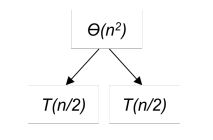
\includegraphics{images/es1_albero.JPG}
            \caption{Rappresentazione dell'albero}
            \label{fig:es1_albero}
        \end{figure}
        
        Si aggiunge un figlio per ogni chiamata ricorsiva effettuata (in questo caso due), tenendo traccia della dimensione del nuovo problema su cui si richiama l’algoritmo (in questo caso n/2 su entrambe le chiamate). Poi si itera il procedimento su ciascuno dei figli fino ad arrivare alle foglie, che corrispondono ai casi base e quindi non hanno figli. Una volta completato l’albero, il costo computazionale è dato dalla somma dei contributi di tutti i livelli .
        
        Otterremo per tanto:
        \begin{equation*}
            2^0\Theta(n^2)\hspace{1cm}2^1\Theta((\frac{n}{2})^2)\hspace{1cm}2^2\Theta((\frac{n}{2^2})^2)\hspace{1cm}2^i\Theta((\frac{n}{2^i})^2)
        \end{equation*}
        All'i-esima iterazione otterremo:
        \begin{equation*}
            \sum^h_{i=0}2^i\frac{n^2}{2^{2i}}=n^2\sum^h_{i=0}(\frac{1}{2})^i=n^2\Theta(1)=\Theta(n^2)
        \end{equation*}
        
        \item $$\begin{cases}T(n)=3T(\frac{n}{2})+\Theta(n)\\T(1)=\Theta(1)\end{cases}$$
            
        \begin{equation*}
            3^0 \Theta(n)\hspace{1cm}3^1 \Theta(\frac{n}{2})\hspace{1cm}3^2 \Theta(\frac{n}{2^2})\hspace{1cm}3^i \Theta(\frac{n}{2^i})
        \end{equation*}
        \begin{equation*}
            \sum^h_{k=0}3^i\Theta(\frac{n}{2^i})=\Theta(n)\sum^h_{i=0}(\frac{3}{2})^i=\Theta(n)\Theta(\frac{3}{2})^{\log(n)}=\Theta(n)\Theta(\frac{3^{\log_2(n)}}{2^{\log_2(n)}})=\Theta(3^{\log_2(n)})
        \end{equation*}
        
    \end{itemize}
\end{example}

\subsection*{Metodo principale}
Questo metodo è molto utile nella pratica e fornisce una soluzione meccanica per le equazioni di ricorrenza della forma:
$$\begin{cases}T(n) = aT(\frac{n}{b}) + \Theta(f(n))\\T(1) = \Theta(1)\end{cases}$$
Dove $a\geq1$, $b>1$ sono delle costanti ed $f(n)$ è una funzione asintoticamente positiva.

\subsubsection{Enunciato del metodo principale}
Il teorema principale può essere enunciato come segue. Dati $a\geq1$, $b > 1$, una funzione asintoticamente positiva $f(n)$ ed un’equazione di ricorrenza della forma:
$\begin{cases}T(n) = aT(\frac{n}{b}) + \Theta(f(n))\\T(1) = \Theta(1)\end{cases}$ vale che:
$$\begin{cases}
    f(n)=O(n^{\log_ba-\epsilon})\hspace{1cm}T(n)=\Theta(n^{\log_ba})\\
    f(n)=\Theta(n^{\log_ba})\hspace{1.35cm}T(n)=\Theta(n^{\log_ba}\log n)\\
    f(n)=\Omega(n^{\log_ba+\epsilon})\hspace{1cm}T(n)=\Theta(f(n))
\end{cases}$$

Con $\epsilon$ che rappresenta una costante $>0$. Nel primo caso si dice che $f$ è polinomialmente dominata. Nel secondo hanno la stessa asintotica. Nel terzo $f$ domina fortemente. E' necessario specificare la constante $\epsilon$ in quanto alcune funzioni della forma $aT(\frac{n}{b}) + \Theta(f(n))$ potrebbero non rientrare in nessuno dei tre casi.

\begin{example}\phantom{}
    \begin{itemize}
        \item $$\begin{cases}T(n) = 2T(\frac{n}{2}) + \Theta(\frac{n}{\log n}))\\T(1) = \Theta(1)\end{cases}$$
        
        Non rientra in nessun caso perchè confrontando
        \begin{equation*}
            n^{\log_ba}=n^{\log_22}=n\hspace{0.5cm}\text{con}\hspace{0.5cm}f(n)=\frac{n}{\log n}
        \end{equation*}
        notiamo che nessun caso è verificato.
        
        \item $$\begin{cases}T(n) = 3T(\frac{n}{2}) + \Theta(n)\\T(1) = \Theta(1)\end{cases}$$
        \begin{equation*}
            n^{\log_23}\hspace{0.5cm}f(n)=n\hspace{1cm}n=O(n^{\log_23-\epsilon})\hspace{1cm}\Theta(n^{\log_23})
        \end{equation*}
        
        \item $$\begin{cases}T(n) = T(\frac{n}{2}) + \Theta(1)\\T(1) = \Theta(1)\end{cases}$$
        \begin{equation*}
            n^{\log_21}=n^0=1\hspace{0.5cm}f(n)=1\hspace{1cm}1=\Theta(1)\hspace{1cm}\Theta(1\log n)
        \end{equation*}
        
        \item $$\begin{cases}T(n) = 2T(\frac{n}{2}) + \Theta(n)\\T(1) = \Theta(1)\end{cases}$$
        \begin{equation*}
            n^{\log_22}=n\hspace{0.5cm}f(n)=n\hspace{1cm}\Theta(n\log n)
        \end{equation*}
        
    \end{itemize}
\end{example}


\subsection*{Metodo della sostituzione}
L’idea alla base di questo metodo è la seguente. Si ipotizza una soluzione per l’equazione di ricorrenza data; Si verifica se essa "funziona" procedendo per induzione. La difficoltà di questo metodo risiede nel fatto che si deve trovare la funzione più vicina alla vera soluzione.

Applichiamo questo metodo a qualche esempio:
\begin{itemize}
    \item $$\begin{cases}T(n) = T(n-1) + \Theta(1)\\T(1) = \Theta(1)\end{cases}$$

    Essendo l'equazione di ricorrenza dell'algoritmo ricorsivo di ricerca sequenziale sappiamo che vale $\Theta(n)$.
    
    Ma in altra maniera proseguiamo nel seguente modo:
    
    $\begin{cases}T(n) \leq T(n-1) + a\\T(1) = b\end{cases}\to\exists c\hspace{0.5cm}T(n)\leq cn$
    
    \textbf{Caso base}: $T(1)=b\leq c*1$ è verificato se prendo $c>b$;\\
    \textbf{Passo induttivo}: $T(n)\leq T(n-1)+a=c(n-1)+a=cn+a-c\leq cn$ per $a-c\leq 0$ e quindi $a\leq c$.
    
    Quindi abbiamo dimostrato che $T(n)=O(n)$.
    
    Non resta che applicare lo stesso ragionamento per dimostrare:
    
    $\begin{cases}T(n) \leq T(n-1) + a\\T(1) = b\end{cases}\to\exists c\hspace{0.5cm}T(n)\geq cn$
    
    Ottenendo infine $T(n)=\Theta(n)$.

    \item $$\begin{cases}T(n) = T(n-1) + T(n-2) +\Theta(1)\\T(0)=T(1)=\Theta(1)\end{cases}$$
    
    Anche di questo algoritmo (calcolo dell'n-esimo numero di Fibonacci ricorsivo) conosciamo il costo computazionale. Ma proviamo a calcolarlo con il metodo dell'induzione:
    \begin{equation*}
        T_1(n)\leq 2T(n-1)+\Theta(1)\hspace{1cm}\text{e}\hspace{1cm}T_2(n)\geq 2T(n-2)+\Theta(1)
    \end{equation*}
    \begin{equation*}
        T_2(n)\leq T(n)\leq T_1(n)
    \end{equation*}
    
    Risolvo $T_1$ ottenendo:
    \begin{equation*}
        T_1=2T(n-1)+\Theta(1)=2[2T(n-2)+\Theta(1)]+\Theta(1)
    \end{equation*}
    \begin{equation*}
        2^2T(n-2)=2^n\Theta(1)=\Theta(2^n)
    \end{equation*}
    
    Risolvendo $T_2$ invece otteniamo $\Theta(2^{\frac{n}{2}})$.
    
    \begin{equation*}
        \Theta(2^\frac{n}{2})\leq T(n)\leq \Theta(2^n)
    \end{equation*}
\end{itemize}

\chapter{Problema dell'ordinamento}
In questo capitolo si affronta l’importante problema dell'ordinamento. Dapprima sono descritti degli algoritmi concettualmente semplici, che hanno
costo computazionale quadratico nella dimensione dell'input. Poi ci si chiede se si possa sperare di trovare un algoritmo più efficiente; a tale
scopo, si fornisce un teorema per cui nessun algoritmo di ordinamento che operi per confronti possa avere costo computazionale inferiore ad un ordine di $n\log n$.

Tutti gli algoritmi che vedremo hanno alcuni aspetti in comune. Si basano su due tipi fondamentali di operazioni: il confronto fra due elementi e lo scambio di due elementi. Inoltre, per semplicità, si suppone che gli n elementi da ordinare siano numeri interi e siano contenuti in un array i cui indici vanno da $0$ a $n-1$. 

\section{Selection sort}
L’algoritmo \textit{selection sort} (ordinamento per selezione) funziona nel seguente modo: cerca il minimo dell'intero array e lo mette in prima posizione; quindi cerca il nuovo minimo nell'array restante, cioè nelle posizioni dalla seconda all'ultima incluse, e lo mette in seconda posizione, e così via. In pratica, dopo l’iterazione i-esima, l’array risulterà suddiviso in due parti: quella di sinistra (di lunghezza $i$) contenente i primi $i$ elementi della sequenza ordinata nel giusto ordine, e quella di destra (di lunghezza $n-i$) contenente gli altri elementi non ordinati.
La formulazione dell'algoritmo è la seguente:
\begin{lstlisting}[language=Python]
    def Selection_Sort(A):
        n=len(A)
        for i in range(n-1)
            m = i
            for j in range(i + 1, n):
                if (A[j] < A[m]):
                    m = j
            A[i],A[m]=A[m],A[i]
\end{lstlisting}
Il costo di questo algoritmo non dipende in alcun modo dalla distribuzione iniziale dei dati nell'array, cioè resta la stessa sia che l’array sia  inizialmente ordinato o no. Essa è:\begin{equation*}\sum^{n-2}_{i=0}n-1-i\hspace{1cm}j=n-1-i\hspace{1cm}\sum^{1}_{j=n-1}j=\Theta(n^2)\end{equation*}


\section{Insertion sort}
L’algoritmo \textit{insertion sort} (ordinamento per inserzione) si effettua “estraendo” l’elemento così da liberare la sua posizione corrente, spostando poi verso destra tutti gli elementi alla sua sinistra (già ordinati) che sono maggiori di esso ed, infine, inserendo l’elemento nella posizione che si è liberata. Alla fine del procedimento l’array risulterà ordinato. La formulazione dell'algoritmo è la seguente:
\begin{lstlisting}[language=Python]
    def Insertion_Sort(A):
        for j in range(1, len(A)):
            x = A[j]
            i = j - 1
            while ((i >= 0)and(A[i]) > x):
                A[i+1] = A[i]
                i = i - 1
            A[i+1] = x
\end{lstlisting}

Valutiamo il costo computazionale dell'algoritmo distinguendo due casi:
\subsubsection{Caso ottimo}
Esso si verifica quando il numero di spostamenti da effettuare è minimo e cioè quando l’array è già ordinato. In tal caso la condizione del while non è mai verificata e quindi:\begin{equation*}\sum^{n-1}_{i=0}\Theta(1)=\Theta(n)\end{equation*}
\subsubsection{Caso pessimo}
Esso si verifica quando il numero di spostamenti da effettuare è massimo e cioè quando l’array in partenza è ordinato in maniera decrescente. Il costo è:\begin{equation*}\sum^{n-1}_{i=0}i=\Theta(n^2)\end{equation*}

\section{Bubble sort}
L’algoritmo \textit{bubble sort} (ordinamento a bolle) ha un funzionamento molto semplice: l’algoritmo ispeziona una dopo l’altra ogni coppia di elementi adiacenti e, se l’ordine dei due elementi non è quello giusto, essi vengono scambiati. L’algoritmo prosegue fino a che non vi sono più coppie di elementi adiacenti nell'ordine sbagliato. La formulazione dell'algoritmo è la seguente:
\begin{lstlisting}[language=Python]
    def Bubble_Sort(A):
        n=len(A)
        for i in range(n-1):
            for j in range (n-i-1):
                if (A[j] > A[j+1]):
                    A[j],A[j+1]=A[j+1],A[j]
\end{lstlisting}
Con questo procedimento il massimo valore viene portato alla fine del vettore, producendo una complessità dell'ordine:
\begin{equation*}
    \sum^{n-1}_{i=0}i=\Theta(n^2)
\end{equation*}


\section*{La complessità del problema dell'ordinamento}
Abbiamo visto che i tre algoritmi di ordinamento precedenti hanno tutti un costo computazionale asintotico che cresce come $\Theta(n^2)$. Una domanda sorge spontanea: si può fare di meglio? E se si, quanto meglio si può fare?
In altre parole, come si fa a stabilire un limite di costo computazionale al di sotto del quale nessun algoritmo di ordinamento basato su confronti fra coppie di elementi possa andare? 

Esiste uno strumento adatto allo scopo, l’albero di decisione. Esso permette di rappresentare tutte le strade che la computazione di uno specifico algoritmo può intraprendere, sulla base dei possibili esiti dei test previsti dall'algoritmo stesso.
Un albero di questo tipo è formato dalle seguenti caratteristiche:
\begin{itemize}
    \item è un albero binario che rappresenta tutti i possibili confronti che vengono effettuati dall'algoritmo; ogni nodo interno ha esattamente due figli;
    \item ogni nodo interno rappresenta un singolo confronto, ed i due figli del nodo sono relativi ai due possibili esiti di tale confronto;
    \item ogni foglia rappresenta una possibile soluzione del problema, la quale è una specifica permutazione della sequenza in ingresso.
\end{itemize}

Eseguire l’algoritmo corrisponde a scendere dalla radice dell'albero alla foglia che contiene la permutazione che costituisce la soluzione. Dunque, la lunghezza del percorso più lungo dalla radice ad una foglia (ossia l’altezza dell'albero binario) rappresenta il numero di confronti che l’algoritmo deve effettuare nel caso peggiore.

Ora, dato che la sequenza di ingresso può avere una qualunque delle sue permutazioni come soluzione, l’albero di decisione deve contenere nelle foglie tutte le permutazioni della sequenza in ingresso, che sono $n!$. D’altra parte, un albero binario di altezza $h$ non può contenere più di $2^h$ foglie, quindi l’altezza $h$ dell'albero di decisione di qualunque algoritmo di ordinamento basato su confronti deve essere tale per cui:
\begin{equation*}
    2^h\leq n!\hspace{1cm}h\leq \log n!
\end{equation*}
Da cui ricaviamo:
\begin{equation*}
    \log n! \leq\log(\frac{n}{2})\frac{n}{2}=\frac{n}{2} \log \frac{n}{2} = \Theta(n\log n)
\end{equation*}

\begin{thm}
    Il costo computazionale di qualunque algoritmo di ordinamento basato su confronti è $\Omega(n \log n)$.
\end{thm}

\section{Mergesort}
L’algoritmo \textit{mergesort} (ordinamento per fusione) è un algoritmo ricorsivo che adotta una tecnica algoritmica detta \textbf{divide et impera}. Essa può essere descritta come segue:
\begin{itemize}
    \item \textbf{divide}: la sequenza di n elementi viene divisa in due sotto-sequenze di n/2 elementi ciascuna;
    \item \textbf{impera}: le due sotto-sequenze di n/2 elementi vengono ordinate ricorsivamente;
    \item \textbf{passo base}: la ricorsione termina quando la sotto-sequenza è costituita di un solo elemento, per cui è già ordinata;
    \item \textbf{combina}: le due sotto-sequenze – ormai ordinate – di n/2 elementi ciascuna vengono “fuse” in un’unica sequenza ordinata di n elementi.
\end{itemize}
Lo pseudocodice dell’algoritmo mergesort è il seguente:
\begin{lstlisting}[language=Python]
def Merge_sort (A, indice_primo, indice_ultimo):
    if (indice_primo < indice_ultimo):
        indice_medio = (indice_primo+indice_ultimo)//2
        Merge_sort (A, indice_primo, indice_medio)
        Merge_sort (A, indice_medio + 1, indice_ultimo)
        Fondi (A, indice_primo, indice_medio, indice_ultimo)
\end{lstlisting}

Vediamone il funzionamento su un problema costituito di 8 elementi, dando per scontato (solo per il momento) il funzionamento della funzione Fondi:
\begin{figure}
    \centering
    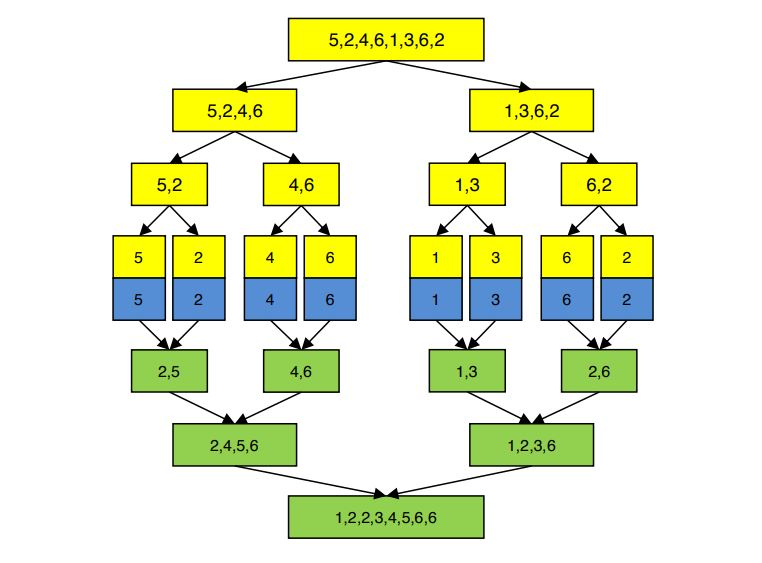
\includegraphics[width = 10cm]{images/mergesort_es.JPG}
    \caption{Procedimento del Merge sort}
    \label{fig:my_label}
\end{figure}

Si osservi che le caselle gialle del disegno corrispondono alle operazioni di suddivisione dell'array in sottoarray, cosa che avviene solo tramite le varie chiamate ricorsive. Le caselle azzurre del disegno invece indicano i casi base e quelle verdi corrispondono alle chiamate della funzione Fondi, le quali restituiscono porzioni di array ordinate sempre più grandi.

Illustriamo ora il funzionamento della fase di fusione:
\begin{lstlisting}[language=Python]
    def Fondi (A; indice_primo, indice_medio, indice_ultimo):
        i,j = indice_primo, indice_medio+1
        B=[]
        while ((i <= indice_medio) and (j <= indice_ultimo))
            if (A[i] <= A[j]):
                B.append(A[i])
                i += 1
            else:
                B.append(A[j])
                j += 1
        while (i <= indice_medio)
            B.append(A[i])
            i += 1
        while (j <= indice_ultimo)
            B.append(A[j])
            j += 1
        for i in range(len(B)):
            A[indice_primo+i] = B[i]
\end{lstlisting}

Essa sfrutta il fatto che le due sotto-sequenze sono ordinate, cosa che rende facile sfruttare un ciclo che scorre partendo dall'inizio delle due sotto-sequenze, confronta i primi elementi alla ricerca del valore minimo da inserire nel vettore. In base al valore trovato (se si trova nella prima sequenza o nella seconda), incrementa l'indice della sotto-sequenza e ripete l'operazione. Alla fine di ciò i due cicli aggiuntivi controllano che non ci siano altri elementi da aggiungere, in caso contrario salva anche quelli nel vettore.
In questo modo abbiamo creato un "vettore copia" che ci permette di salvare la sequenza ordinata. 

\subsubsection{Costo del Mergesort}
Analizziamo il costo dell'operazione di fusione e poi quella dell'algoritmo mergesort. 

Nella fusione si effettuano un ciclo while, nel quale per ogni elemento di ciascuna delle due sotto-sequenze si compie un numero costante di operazioni. Il costo computazionale del while è individuato dal numero di iterazioni: poiché si scorre un array di dimensione $\frac{n}{2}$ quindi $\Theta(n)$.

L’equazione di ricorrenza del mergesort è di conseguenza: 
$$\begin{cases}
    T(n) = 2T(\frac{n}{2}) + \Theta(n)\\
    T(1) = \Theta(1)
\end{cases}$$

Essa ricade nel caso 2 del teorema principale, la cui soluzione è $T(n) = \Theta(n \log n)$.

\section*{Timsort}
Nonostante il Merge Sort funzioni in tempo $O(n \log n)$ mentre l'Insertion Sort in $O(n^2)$, i fattori costanti sono tali che l’Insertion Sort è più veloce del Merge Sort per valori piccoli di n. Quindi, ha senso usare l’Insertion Sort dentro il Merge Sort quando i sottoproblemi diventano sufficientemente piccoli.

L'algoritmo descritto nel testo può essere il seguente:
\begin{lstlisting}[language=Python]
def Merge_Insertion (A,k, primo, ultimo, dim):
    if dim>k:
        medio =(primo+ultimo)//2
        Merge_Insertion (A,k, primo, medio, medio-primo+1)
        Merge_Insertion (A,k, medio+1, ultimo, ultimo-medio)
        Fondi(A, primo, medio, ultimo)
    else: InsertionSort(primo, ultimo)
\end{lstlisting}

L’equazione di ricorrenza associata a questa funzione è:
$$\begin{cases}
    T(n)=2T(\frac{n}{2})+ \Theta(n)\\
    T(k)= \Theta(k^2)
\end{cases}$$
Che può essere risolta con il metodo iterativo che dopo i passi si presenta come:
\begin{equation*}
    T(n)=2^iT(\frac{n}{2^i})+\sum^{i-1}_{j=0}2^j\Theta(\frac{n}{2^j})\hspace{1cm}\frac{n}{2}\approx k\hspace{1cm}i=\log\frac{n}{k}
\end{equation*}
\begin{equation*}
    T(n)=2^{\log\frac{n}{k}} \Theta(k^2) + \Theta(n) \sum_{j=0}^{\log\frac{n}{k}+1}1 = \Theta(\frac{n}{k}k^2) + \Theta(n)\log\frac{n}{k}
\end{equation*}
che è dell’ordine di $n\log n$ se $k=O(\log n)$.


\section{Quicksort}
L’algoritmo \textit{quicksort} (ordinamento veloce) è un algoritmo che ha una caratteristica molto interessante: nonostante abbia un costo che nel caso peggiore è $O(n^2)$, nella pratica si rivela spesso la soluzione migliore per grandi valori di n perché: il suo tempo di esecuzione atteso è $\Theta(n \log n)$; i fattori costanti nascosti sono molto piccoli; permette l’ordinamento “in loco”.
Anche il quicksort sfrutta la tecnica algoritmica del divide et impera:
\begin{itemize}
    \item \textbf{divide}: nella sequenza di $n$ elementi viene selezionato un elemento detto \textit{pivot}. La sequenza viene quindi divisa in due sotto-sequenze: la prima delle due contiene elementi minori o uguali del pivot, la seconda contiene elementi maggiori o uguali del pivot;
    \item \textbf{passo base}: la ricorsione procede fino a quando le sotto-sequenze sono costituite da un solo elemento;
    \item \textbf{impera}: le due sotto-sequenze vengono ordinate ricorsivamente;
    \item \textbf{combina}: non occorre alcuna operazione poiché la sequenza è già ordinata.
\end{itemize}

Lo pseudocodice dell’algoritmo quicksort è il seguente:
\begin{lstlisting}[language=Python]
    def Quick_sort (A, indice_primo, indice_ultimo):
        if (indice_primo < indice_ultimo):
            indice_medio = Partiziona (A, indice_primo, indice_ultimo)
            Quick_sort (A, indice_primo, indice_medio-1)
            Quick_sort (A, indice_medio+1, indice_ultimo)
\end{lstlisting}

\verb|Partiziona| seleziona il valore dell'elemento più a destra e lo usa come pivot per partizionare la sequenza in tre regioni: alla fine del procedimento la regione di sinistra conterrà solo elementi minori o uguali al pivot, quella di destra conterrà solo elementi maggiori o uguali al pivot, e quella centrale, formata da un solo elemento, contenente il pivot.
\begin{lstlisting}[language=Python]
    def Partiziona (A, indice_primo, indice_ultimo):
        pivot = indice_ultimo //scelta arbitraria
        i = indice_primo-1
        for j in range(indice_primo,indice_ultimo):
            if (A[j]<=A[pivot]):
                i+=1
                A[i],A[j]=A[j],A[i]
        A[i+1],A[indice_ultimo]=A[indice_ultimo],A[i+1]
        return i+1
\end{lstlisting}

Prima di analizzare il costo computazionale del Quicksort, vediamo il suo funzionamento su un piccolo esempio.
\begin{example}
    Sia dato l’array $A=[2,8,7,1,3,5,6,4]$; la funzione \verb|Partiziona| modifica l’array in modo che esso divenga $A=[2,1,3,4,7,5,6,8]$ e restituisce l’indice 3 (corrispondente al pivot con valore 4). A questo punto, la funzione \verb|Quick|\textunderscore\verb|sort| viene richiamata ricorsivamente sui due sotto-array $[2,1,3]$ e $[7,5,6,8]$.
    
    Proseguendo le chiamate sui sotto-array che via via scaturiscono dai vari valori che vengono restituiti dalla funzione \verb|Partiziona|, si giunge, infine, all'array ordinato.
    
    \begin{figure}[H]
        \centering
        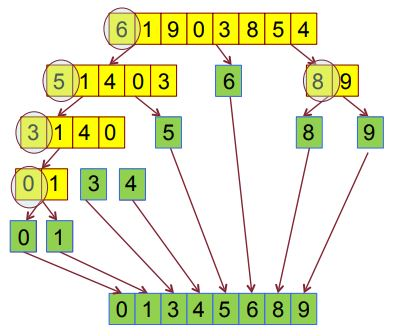
\includegraphics[width = 8cm]{images/quick-sort.JPG}
        \caption{Quick sort}
        \label{fig:quick_sort}
    \end{figure}
\end{example}

Per il costo computazionale, l’equazione di ricorrenza del quicksort va dunque espressa come segue:
$$\begin{cases}T(n) = T(k) + T(n-1-k) + \Theta(n)\\T(1) = \Theta(1)\end{cases}\hspace{0.5cm}0 \leq k \leq n-1$$
che non sappiamo come risolvere con alcuno dei metodi illustrati precedentemente. Possiamo però valutarla in casi specifici: nel caso peggiore, in quello migliore e in quello medio.
\subsubsection{Caso peggiore}
Il caso peggiore è quello in cui, ad ogni passo, la dimensione di uno dei due sotto-problemi da risolvere è nulla. In tale situazione l’equazione di ricorrenza è:
\begin{equation*}T(n) = T(n - 1) + \Theta(n)\end{equation*}
Applicando il metodo dell'albero: otteniamo un albero degenere\footnote{Un albero binario si dice degenere se ha n nodi e altezza n-1, cioè se ogni nodo interno ha un solo figlio.}. Il costo dei nodi decresce linearmente da n (nella radice) ad 1 (nell'unica foglia). Quindi il costo computazionale è:
\begin{equation*}T(n)=\Theta\sum^n_{i=1}i=\Theta(n^2)\end{equation*}
\subsubsection{Caso migliore}
Si può dimostrare che il caso caso migliore è quello in cui \textit{Partiziona} ottiene due sotto-problemi il più bilanciati possibile, e in questo caso la ricorrenza diviene:
\begin{equation*}T(n)=2T(\frac{n-1}{2})+\Theta(n)\end{equation*} 
che, similmente a come già visto per il mergesort, ha soluzione $T(n) = \Theta(n\log n)$.
\subsubsection{Caso medio}
Valutiamo il costo computazionale del caso medio, nell'ipotesi che il valore del pivot suddivida con uguale probabilità $\frac{1}{n}$.
Partendo da:
$$\begin{cases}
    T(n)=\frac{1}{n}[\sum^{n-1}_{k=0}(T(k)+T(n-1-k))]+\Theta(n)\\
    T(0)=T(1)=\Theta(1)
\end{cases}$$
Per ogni valore di $k=0,1,...,n-1$ il termine $T(i)$ compare due volte nella sommatoria, la prima quando $k=i$ e la seconda quando $k=n-1-i$.
Valutiamo dunque il valore di:
\begin{equation*}
    T(n)=\frac{2}{n}\sum^{n-1}_{k=0}T(k)+\Theta(n)
\end{equation*}
Utilizziamo il metodo di sostituzione, e quindi eliminiamo innanzitutto la notazione asintotica:
\begin{equation*}
    T(n)=\frac{2}{n}[\sum^{n-1}_{k=0}T(k)]+an
\end{equation*}
Ipotizziamo ora la soluzione $T(n) \leq cn\log n$. E calcoliamo il caso base $T(2)=\frac{2}{2}+2a=2a\leq2c$, risulta vera per $c\geq a$.
Per il passo induttivo possiamo scrivere:
\begin{equation*}
    T(n)\leq \frac{2}{n}[\sum^{n-1}_{k=2}ck\log k]+an=\frac{2c}{n}[\sum^{n-1}_{k=2}k\log k]+an=\frac{2c}{n}[\sum^{n-1}_{k=1}k\log k]+an
\end{equation*}
Essendo $\sum^{n-1}_{i=1}i\log i$ una serie nota che risulta essere $\leq \frac{n^2}{n}\log n-\frac{n^2}{8}$, diciamo che:
\begin{equation*}
    \frac{2c}{n}[\sum^{n-1}_{k=1}k\log k]+an\leq\frac{2c}{n}(\frac{n^2}{2}\log n-\frac{n^2}{8})+an=cn\log n-\frac{cn}{4}+an
\end{equation*}
Volendo $-\frac{cn}{4}+an\leq cn\log n$ minore di zero, ovvero per $c\geq4a$ otteniamo:
\begin{equation*}
    cn\log n-\frac{cn}{4}+an\leq cn\log n
\end{equation*}


\section{Heapsort}
L’algoritmo \textit{heapsort} è un algoritmo di ordinamento piuttosto complesso che esibisce ottime caratteristiche. Inoltre, questo algoritmo è l’occasione per iniziare a illustrare un concetto molto importante, quello di struttura dati. Sfrutta, infatti, una opportuna organizzazione dei dati che garantisce una o più specifiche proprietà, il cui mantenimento è essenziale per il corretto funzionamento dell'algoritmo.
\subsubsection{Che cos'è l'heap?}
L'heap (mucchio) è una struttura dati, nello specifico è un albero binario completo o quasi completo, ossia un albero binario in cui
tutti i livelli sono pieni, tranne l’ultimo.

\begin{wrapfigure}{r}{0.2\textwidth}
  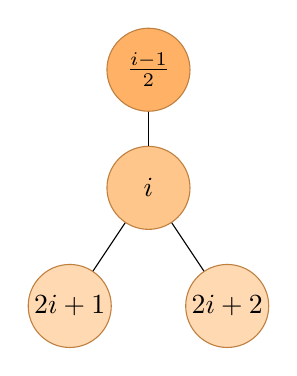
\begin{tikzpicture}
  [level distance=15mm,
   every node/.style={draw=brown,fill=orange!60,circle,inner sep=1pt, minimum size=3em},
   level 1/.style={sibling distance=20mm,minimum size=2em,nodes={fill=orange!45}},
   level 2/.style={sibling distance=20mm,minimum size=.5em,nodes={fill=orange!30}},
   level 3/.style={sibling distance=5mm,nodes={fill=orange!25}}]
  \node {$\frac{i-1}{2}$}
     child {node {$i$}
       child {node {$2i+1$}}
       child {node {$2i+2$}}
     };
\end{tikzpicture}
\end{wrapfigure}

Il modo più naturale per memorizzare questa struttura dati è utilizzare un array. Ogni nodo dell'albero binario corrisponde a uno e un solo elemento dell'array, la radice dell'albero corrisponde ad $A[0]$. 
Il figlio sinistro del nodo che corrisponde all'elemento $A[i]$, se esiste, corrisponde all'elemento $A[2i+1]$, mentre quello destro corrisponde all'elemento $A[2i + 2]$. Il padre del nodo dell'elemento $A[i]$ corrisponde all'elemento $A[\frac{i-1}{2}]$.

\begin{figure}
    \centering
    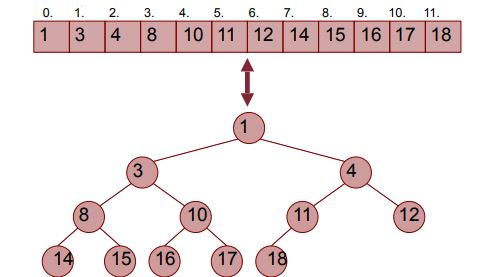
\includegraphics[width = 10cm]{images/heap.JPG}
    \caption{Esempio di heap}
    \label{fig:heap}
\end{figure}

Le funzioni che implementa questa particolare struttura sono:
\begin{itemize}
    \item La \textbf{creazione} dell'heap che avviene in tempo $O(n)$;
    \item L'\textbf{estrazione del minimo} che avviene in tempo $O(\log A)$ (A è la dimensione dell'heap$\backslash$ array);
    \item L'\textbf{inserimento} di un valore che avviene in tempo $O(\log A)$ (A è la dimensione dell'heap$\backslash$ array).
\end{itemize}
In particolare queste funzioni vengono gestite dai seguenti metodi:
\begin{lstlisting}[language=Python]
    import heapq
    heapify(A)
    x = heappop(A)
    heappush(A,x)
\end{lstlisting}


Ora non sarà difficile capire l'idea dietro l’algoritmo dell’heapsort:
\begin{itemize}
    \item si organizzano gli elementi in A da ordinare come heap minimo;
    \item si estraggono gli elementi dell'heap uno alla volta per inserirli in un nuovo vettore B inizialmente vuoto;
    \item si restituisce il vettore B.
\end{itemize}

Ad ogni estrazione si estrae da A il valore minimo quindi gli elementi finiranno
nel nuovo vettore in ordine crescente.
\begin{lstlisting}[language=Python]
    import heapq
    def Heap_Sort(A):
        heapq.heapify(A)
        B=[]
        while A:
            B.append(heapq.heappop(A))
    return B
\end{lstlisting}
La complessità temporale dell'algoritmo dovrebbe risultare $\Theta(n\log n)$, ma in questa specifica versione l’algoritmo non ordina in loco e lo spazio di lavoro è $O(n^2)$ a causa dell’utilizzo del vettore $B$.

\subsubsection{Heappop()}
I passaggi da seguire per l'implementazione della funzione \verb|Heappop()| sono:
\begin{itemize}
    \item salviamo in una variabile il minimo presente in $A[0]$; 
    \item ricopiamo in $A[0]$ l’ultimo elemento $A[n-1]$ dell’heap e cancelliamo da $A$ l’ultimo elemento;
    \item ci ritroviamo con un heap dove l’unico elemento fuori posto è quello alla radice e possiamo riaggiustare l’heap con una sola chiamata di \verb|heapify| sull’elemento in posizione 0;
    \item restituiamo l’elemento.
\end{itemize}

\begin{lstlisting}[language=Python]
    def Heappop(A):
        x = A[0]
        A[0] = A[len(A)-1]
        A.pop()
        Heapify(A,0)
        return x
\end{lstlisting}
La complessità di questa funzione, per via dell'invocazione di \verb|Heapify()|, risulta essere $O(\log n)$.

\subsubsection{Heappush()}
I passaggi da seguire per l'implementazione della funzione \verb|Heappush()|:
\begin{itemize}
    \item aggiungiamo l’elemento x all'ultimo posto dell'heap;
    \item fino a che non risulta maggiore del padre o raggiunge la radice facciamolo risalire nell'heap.
\end{itemize}

\begin{lstlisting}[language=Python]
    def Heappush(A,x):
        A.append(x)
        i = len(A)-1
        while i>0 and A[i]<A[(i-1)//2]:
            A[i], A[(i-1)//2] = A[(i-1)//2], A[i]
            i = (i-1)//2
\end{lstlisting}

La complessità della procedura dipende dal numero di iterazioni del \verb|while| e questo numero è $O(\log n)$.

\subsubsection{Heapify()}
L’algoritmo di \verb|Heapify| si avvale di una funzione ausiliaria \verb|Heapify1|, necessaria per il suo corretto funzionamento. La funzione \verb|Heapify1| ha lo scopo di mantenere la proprietà di heap, sotto l’ipotesi che nell'albero su cui viene fatta lavorare sia garantita la proprietà di heap per entrambi i sotto-alberi (sinistro e destro) della radice. Di conseguenza l’unico nodo che può violare la proprietà di heap è la radice dell'albero, che può essere minore di uno o di entrambi i figli. La funzione opera sulla radice confrontandola coi suoi figli e, se necessario, la scambia col minore dei suoi figli. Dopo che lo scambio si verifica se la violazione si è trasferita sul figlio scambiato si ripete ricorsivamente l’operazione su tale nodo.

\begin{lstlisting}[language=Python]
    def Heapify1(A, i):
        n = len(A)
        L = 2*i+1; R = 2*i+2
        indice_min = i
        if L < len(A) and A[L] < A[indice_min]:
            indice_min = L
        if R < len(A) and A[R] < A[indice_min]:
            indice_min = R
        if indice_min != i:
            A[i], A[indice_min] = A[indice_min], A[i]
            Heapify1(A, indice_min)
\end{lstlisting}

Calcoliamo ora il costo computazionale di \verb|Heapify1|. Dalle chiamate ricorsive otteniamo $T(n) = T(n') + \Theta(1)$ dove $n$ è il numero di nodi del sotto-albero radicato in $i$ e dove $n'$ è il numero di nodi del sotto-albero di che ha più nodi. I sotto-alberi della radice non possono avere più di $\frac{2n}{3}$ nodi. Sia $n' = 2^h-1$ il numero di nodi nel sotto-albero di sinistra.
\begin{equation*}
    n'=2^{h+1}-1-\frac{2^h}{2}=\frac{3*(2^h-1)+1}{2}=\frac{3n'+1}{2}\hspace{1cm}n'=\frac{2n-1}{3}<\frac{2n}{3}
\end{equation*}
Quindi l’equazione di ricorrenza diventa $T(n) \leq T(\frac{2n}{3})+\Theta(1)$, che ha soluzione: $T(n)=O(\log n)$.\\

Possiamo ora passare all'analisi di \verb|Heapify|. \verb|Heapify| serve per trasformare qualunque vettore contenente elementi in uno heap, chiamando ripetutamente \verb|Heapify1| sugli opportuni nodi dello heap. Inoltre poiché \verb|Heapify1| presuppone che entrambi i sotto-alberi della radice siano heap, deve essere chiamata scorrendo l’albero per livelli dal basso verso l’alto (quindi, sul vettore, da destra a sinistra). Ogni foglia è già uno heap, quindi possiamo chiamare \verb|Heapify| a partire dal nodo interno più a destra.

\begin{lstlisting}[language=Python]
    def Heapify(A):
        for i in range((len(A)-2)//2,-1,-1):
            Heapify1(A, i)
\end{lstlisting}

La funzione \verb|Heapify| effettua $n$ chiamate di \verb|Heapify1|, che sappiamo avere ciascuna costo $O(\log n)$, quindi: $T(n)=O(n\log n)$.

Non resta che dimostrare che $T(n)=\Theta(n)$.
Considerando un heap di altezza $h$. Nell'heap a livello $i$ ci sono al più $2^i$ nodi, quindi il numero di nodi dell’heap che sono radice di un sotto-albero di altezza $i$ sono $2^{h-1}=\frac{2^h}{2^i}$. Il tempo richiesto da \verb|Heapify| applicata ad un nodo che è radice di un sotto-albero di altezza $i$ è $O(i)$. Quindi possiamo scrivere:
\begin{equation*}
    T(n)\leq\sum^h_{i=1}2^{h-i}O(i)=O(2^h\sum^h_{i=1}\frac{i}{2^i})=O(2^h\sum^h_{i=1}(\frac{3}{4})^i)
\end{equation*}
perchè $\frac{i}{2^i}<(\frac{3}{4})^i$. Quindi otteniamo $T(n)=O(2^h)+O(1)=O(n)$.

\section*{Ordinamenti stabili}
Un algoritmo di ordinamento si dice stabile se mantiene l'ordine relativo per gli elementi che hanno chiavi uguali. In altre parole, se due elementi hanno la stessa chiave, un algoritmo di ordinamento stabile garantirà che l'elemento che compare prima nella lista originale venga posizionato prima nella lista ordinata. Al contrario, un algoritmo di ordinamento non stabile può riordinare gli elementi con chiavi uguali in modo imprevedibile.

Ad esempio l'algoritmo di SelectionSort non è stabile. Per convincersene basta considerare cosa accade quando si ordina con questo metodo la lista di tre elementi $[2,2,1]$, si ottiene il la lista ordinata $[1,2,2]$ ma l'ordinamento originario dei due elementi uguali risulta invertito. Degli algoritmi di ordinamento passati in rassegna non sono stabili gli algoritmi di SelectionSort, QuickSort ed HeapSort. Sono stabili gli algoritmi di BubbleSort, InsertionSort, MergeSort e TimSort. 

\section*{Ordinamento in tempo lineare}
\textit{È possibile ordinare n elementi in un tempo inferiore a $\Omega(n\log n)$?}
Il teorema che stabilisce una limitazione inferiore al costo degli algoritmi di ordinamento sembrerebbe dire di no; in realtà la risposta è sì, purchè l’algoritmo di ordinamento non sia basato sui confronti fra elementi poiché, in tal caso, come abbiamo visto nessun algoritmo può scendere sotto tale limite.

\section{Counting Sort}
Un esempio è il \textit{counting sort} (algoritmo basato sul conteggio). Esso opera sotto l’assunzione che ciascuno degli $n$ elementi da ordinare sia un intero di valore compreso in un intervallo $[0..k]$ ed ha un costo di $\Theta(n+k)$. Se $k = O(n)$ allora l’algoritmo ordina $n$ elementi in tempo lineare, cioè $\Theta(n)$. L’idea è quella di fare in modo che il valore di ogni elemento della sequenza
determini direttamente la sua posizione nella sequenza ordinata. Questo semplice schema deve essere leggermente complicato per gestire l’eventualità che nella sequenza da ordinare vi siano più elementi con lo stesso valore o manchi un qualche valore.
Oltre all’array A che contiene gli n elementi da ordinare, usiamo un array C di appoggio, contenente k celle.
\begin{lstlisting}[language=Python]
    def Counting_sort(A)
        k=max(A)
        n=len(A)
        C=[0]*(k+1)
        for j in range(n):
            C[A[j]]+= 1
        j=0
        for i in range(k)
            while (C[i] > 0)
                A[j]=i
                j+= 1
                C[i]-= 1
\end{lstlisting}

La prima istruzione calcola il massimo dell'array A e costa, quindi, $\Theta(n)$. L’ inizializzazione a 0 dell'array $C$ costa $\Theta(k)$. Il primo ciclo conta, per ciascun indice di $C$, il numero di elementi di $A$ aventi tale valore. Il secondo ciclo scandisce l’array $C$ e, al suo interno, per ogni valore di $i$, un ciclo \verb|while| scrive $C[i]$ copie di $i$ sull’array $A$. Il numero complessivo di iterazioni del ciclo \verb|while| è pari alla somma dei valori contenuti in $C$, che è esattamente $n$, quindi il costo computazionale è:
\begin{equation*}
    \Theta(n) + \Theta(k) + \Theta(n) + \Theta(k+n) = \Theta(max(k,n)) = \Theta(n) \text{ se }k = \Theta(n).     
\end{equation*}

Segue un piccolo esempio del funzionamento dell’algoritmo di Counting Sort. Sia dato l’array $A = [2, 5, 1, 2, 3, 3, 5, 0, 3, 1]$. In questo caso $n = 10$ e $k=5$. Dopo l’esecuzione del ciclo \verb|for j in range(n)|, l’array $C$ contiene i seguenti valori: $C = [1, 2, 2, 3, 0, 2]$ ed, ovviamente, risulta che la somma dei valori contenuti in $C$ è proprio pari ad $n$. A questo punto, è facile ricostruire l’array $A$ ordinato, scrivendo dapprima 3 occorrenze del valore 1, poi 2 occorrenze del valore 2, e così via, fino alla fine dell’array $C$: $A = [0, 1, 1, 2, 2, 3, 3, 3, 5, 5]$.

\section{Bucket sort}
Un altro algoritmo interessante, che ha costo computazionale medio lineare, è il \textit{bucket sort}. Come il counting sort, il bucket sort è efficiente perché fa delle ipotesi sull'input. In particolare, assume che gli $n$ valori dati in input da ordinare siano equamente distribuiti in un intervallo $[1..k]$, e non c’è alcuna ipotesi su $k$.

L’idea del bucket sort consiste nel dividere l’intervallo [$1..k]$ in $n$ sotto-intervalli di uguale ampiezza $\frac{k}{n}$, detti bucket. A causa dell’ipotesi di equi-distribuzione, non ci si aspetta che molti valori dell'input cadano in ciascun intervallo, anzi in media essi saranno in numero costante.
Il bucket sort introduce un array ausiliario di lunghezza $n$ di array, ciascuno delle quali conterrà tutti gli elementi dati in input che cadono in un certo sotto-intervallo; più in dettaglio, un bucket i conterrà tutti i valori compresi tra $\frac{(i-k)}{n}$.
\begin{lstlisting}
    def Bucket_sort(A,k):
        M=max(A)
        k=min(k,M+1,len(A))
        B=[[]for _ in range(k)]
        for x in A:
            B[int (x*k/(M+1))].append(x)
        for i in range(k):
            B[i].sort()
        R=[]
        for i in range(k):
            R.extend(B[i])
        return R
\end{lstlisting}
Per quanto riguarda il costo computazionale dell'algoritmo di bucket sort, è chiaro che esso dipende fortemente dalla lunghezza delle liste $B[i]$. Poiché, come abbiamo già evidenziato, tale lunghezza è mediamente costante, è facile vedere che il costo computazionale medio di questo algoritmo è lineare. Invece, nel caso peggiore, esso sarà quadratico.

\begin{figure}[ht]
    \centering
    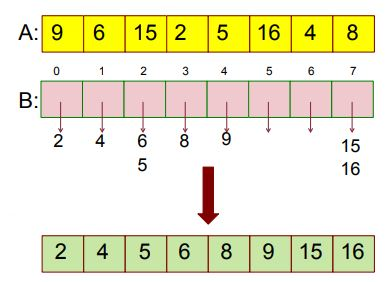
\includegraphics[width = 7cm]{images/bucket_sort.JPG}
    \caption{Bucket sort}
    \label{fig:bucket_sort}
\end{figure}



\chapter*{Esercizi svolti}
\addcontentsline{toc}{chapter}{Esercizi svolti}
\begin{exercise}[Problema della ricerca]
    Sia dato un vettore di interi \verb|A| e due valori $a$ e $b$ con $a\leq b$, il problema è quello di sapere quanti elementi di \verb|A| sono compresi nell'intervallo chiuso $[a,b]$.
    \begin{enumerate}
        \item Si progetti un algoritmo per risolvere tale problema su qualsiasi vettore \verb|A|;
        \item Si progetti un algoritmo più efficiente del precedente assumendo che \verb|A| sia già ordinato e che contenga solo valori distinti.
    \end{enumerate}
    
    Per il primo punto scorro il vettore e conto gli elementi inclusi nell'intervallo $[a,b]$.
    
    \begin{lstlisting}[language=Python]
        def Conta_in_Intervallo(A,a,b):
            cont = 0
            for i in range(len(A)):
                if a<=A[i]<=b:
                    cont += 1
            return cont
    \end{lstlisting}
    
    Costo dell'algoritmo è $\Theta(n)$.\\
    
    Per il secondo punto cerco $a$ e $b$ nel vettore con la ricerca binaria. Serve una piccola modifica all'algoritmo di ricerca binaria. Basta aggiungere \verb|return m|. In questo modo per il valore m restituito possono accadere tre cose:
    \begin{itemize}
        \item $A[m] = v$. In questo caso $v$ è in $A$ ed $m$ è la sua posizione;
        \item $A[m] < v$. In questo caso $v$ non è in $A$ ed è $m$ la posizione dell'elemento minore di $v$ più a destra presente in $A$;
        \item $A[m] > v$. In questo caso $v$ non è in $A$ ed è $m$ la posizione dell'elemento maggiore di $v$ più a sinistra presente in $A$.
    \end{itemize}

    \begin{lstlisting}[language=Python]
        def Conta_in_Intervallo_ordinato(A,a,b):
            ind_a=ricerca_binaria_modificata(A,a)
            if A[ind_a]<a: ind_a+=1
            ind_b=ricerca_binaria_modificata(A,b)
            if A[ind_b]>b: ind_b-=1
            return ind_b-ind_a+1
    \end{lstlisting}
    Siamo così riusciti a risolvere il problema in tempo $\Theta(\log n)$.
\end{exercise}
 
 \begin{exercise}[Equazioni ricorsive]
    Calcolare la complessità della seguente equazione ricorsiva:
    $$\begin{cases}T(n)=T(\frac{n}{3})+T(\frac{2n}{3})+\Theta(n)\\T(1)=\Theta(1)\end{cases}$$
    In questo tipo di problemi vogliamo ottenere una forma del tipo:
    \begin{equation*}T_1(n)\leq T(n)\leq T_2(n)\hspace{1cm}T_1(n)=\Omega\hspace{1cm}T_2(n)=O\end{equation*}
    Scriviamo:
    \begin{equation*}
        T_1(n)=2T(\frac{n}{3})+\Theta(n)
    \end{equation*}
    applicando il metodo principale otteniamo $n=\Omega(n^{\log_32+\epsilon})$ con risultato $\Theta(n)$.
    
    Scriviamo, invece:
    \begin{equation*}
        T_2(n)=2(\frac{2n}{3})+\Theta(n)
    \end{equation*}
    che con il metodo principale ci rende $n=O(n^{\log_\frac{3}{2}2-\epsilon})$ con risultato $\Theta(n^{\log_\frac{3}{2}2})$.
     \begin{equation*}
         \Omega(n)\leq T(n)\leq O(n^{\log_\frac{3}{2}2})
     \end{equation*}
     Notiamo che con questo metodo non riusciamo ad ottenere il valore effettivo della complessità asintotica, per tanto proviamo con il metodo dell'albero.
     \begin{center}
     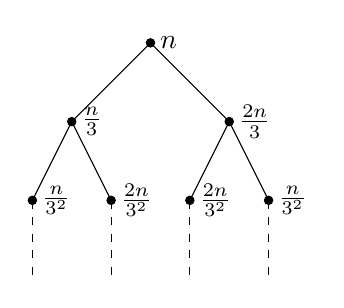
\begin{tikzpicture}
        \draw[] (0,0) -- (-1,-1);\draw[] (0,0) -- (1,-1);\filldraw[black] (0,0) circle (1.5pt) node[anchor=west]{$n$};
        \draw[] (-1,-1) -- (-1.5,-2);\draw[] (-1,-1) -- (-0.5,-2);\filldraw[black] (-1,-1) circle (1.5pt) node[anchor=west]{$\frac{n}{3}$};
        \draw[] (1,-1) -- (1.5,-2);\draw[] (1,-1) -- (0.5,-2);\filldraw[black] (1,-1) circle (1.5pt) node[anchor=west]{$\frac{2n}{3}$};
        \filldraw[black] (-1.5,-2) circle (1.5pt) node[anchor=west]{$\frac{n}{3^2}$};\filldraw[black] (-0.5,-2) circle (1.5pt) node[anchor=west]{$\frac{2n}{3^2}$};
        \filldraw[black] (1.5,-2) circle (1.5pt) node[anchor=west]{$\frac{n}{3^2}$};\filldraw[black] (0.5,-2) circle (1.5pt) node[anchor=west]{$\frac{2n}{3^2}$};
        \draw [dashed] (1.5,-2) -- (1.5,-3);\draw [dashed] (-0.5,-2) -- (-0.5,-3);
        \draw [dashed] (-1.5,-2) -- (-1.5,-3);\draw [dashed] (0.5,-2) -- (0.5,-3);
     \end{tikzpicture}
     \end{center}
     Sommando i costi in ogni fila di nodi otteniamo sempre $\Theta(n)$. Ma va aggiunto che i rami hanno altezze diverse:
     \begin{itemize}
         \item[] Ramo più corto: $\frac{n}{3^i}\approx1\hspace{0.5cm}n\approx3^i\hspace{0.5cm}i\approx\log_3n$;
         \item[] Ramo più lungo: $\frac{2n}{3^i}\approx1\hspace{0.5cm}n\approx\frac{3}{2}^i\hspace{0.5cm}i\approx\log_\frac{3}{2}n$.
     \end{itemize}
     Ottenendo così come risultato:\begin{equation*}\Theta(n)\log_3n\leq T(n)\leq \Theta(n)\log_\frac{3}{2}n\hspace{1cm}\Theta(n\log n)\leq T(n)\leq \Theta(n\log n)\end{equation*}\begin{equation*}T(n)=\Theta(n\log n)\end{equation*}
 \end{exercise}